%% Ca2+ imaging material removed from 2026_Atp1a3.tex for the bioRxiv version
%% Kept here verbatim for the planned follow-up paper.

%%%%%%%% RESULTS SECTION %%%%%%%%
\subsection{Ca2\textsuperscript{2+} imaging identifies altered sensorimotor responses and abnormal bursting activity in the \emph{atp1a3a} mutant forebrain}


\begin{figure}
\begin{center}
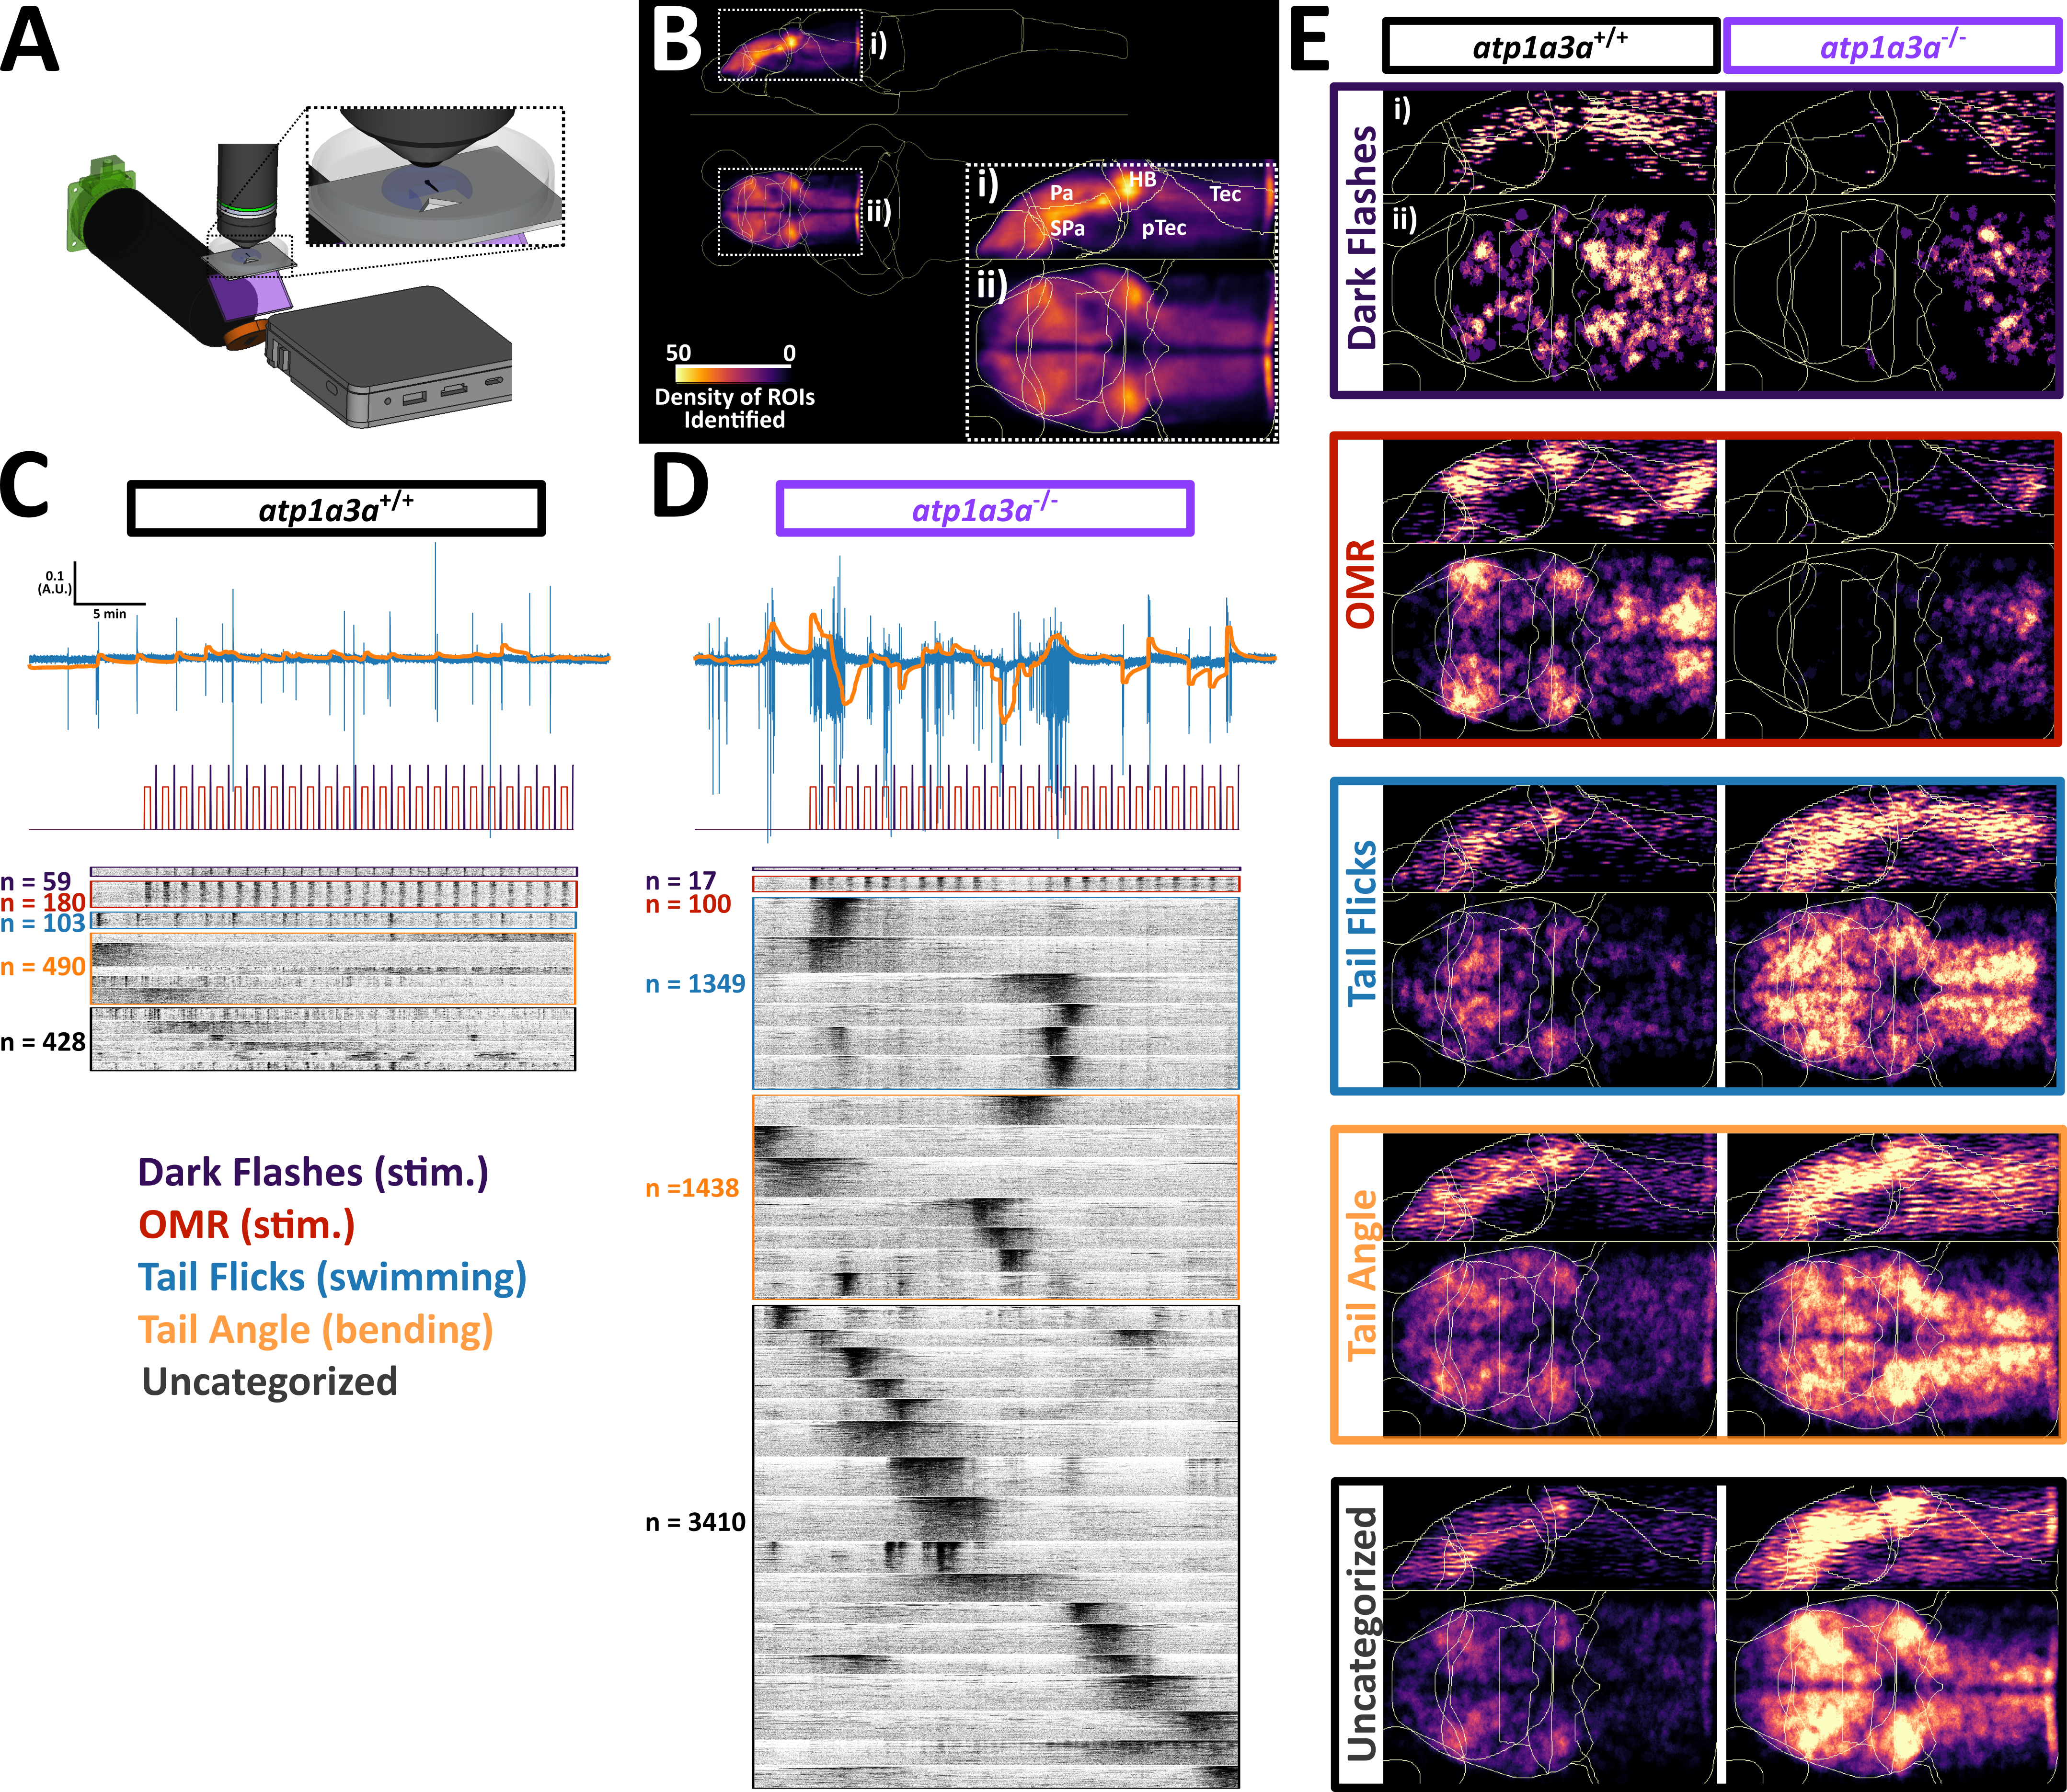
\includegraphics[width=0.9 \linewidth]{Figures/Figure_Ca2Imaging.png}


\caption{\textbf{Ca\textsuperscript{2+} imaging of \emph{atp1a3a} mutant forebrain activity}\\
\textbf{A)} asdfadfasdf
}


\label{fig:6}


\figsupp[Regional quantification of identified neurons across genotypes.]
{Regional quantification of identified neurons across genotypes..
\textbf{A)} 
}{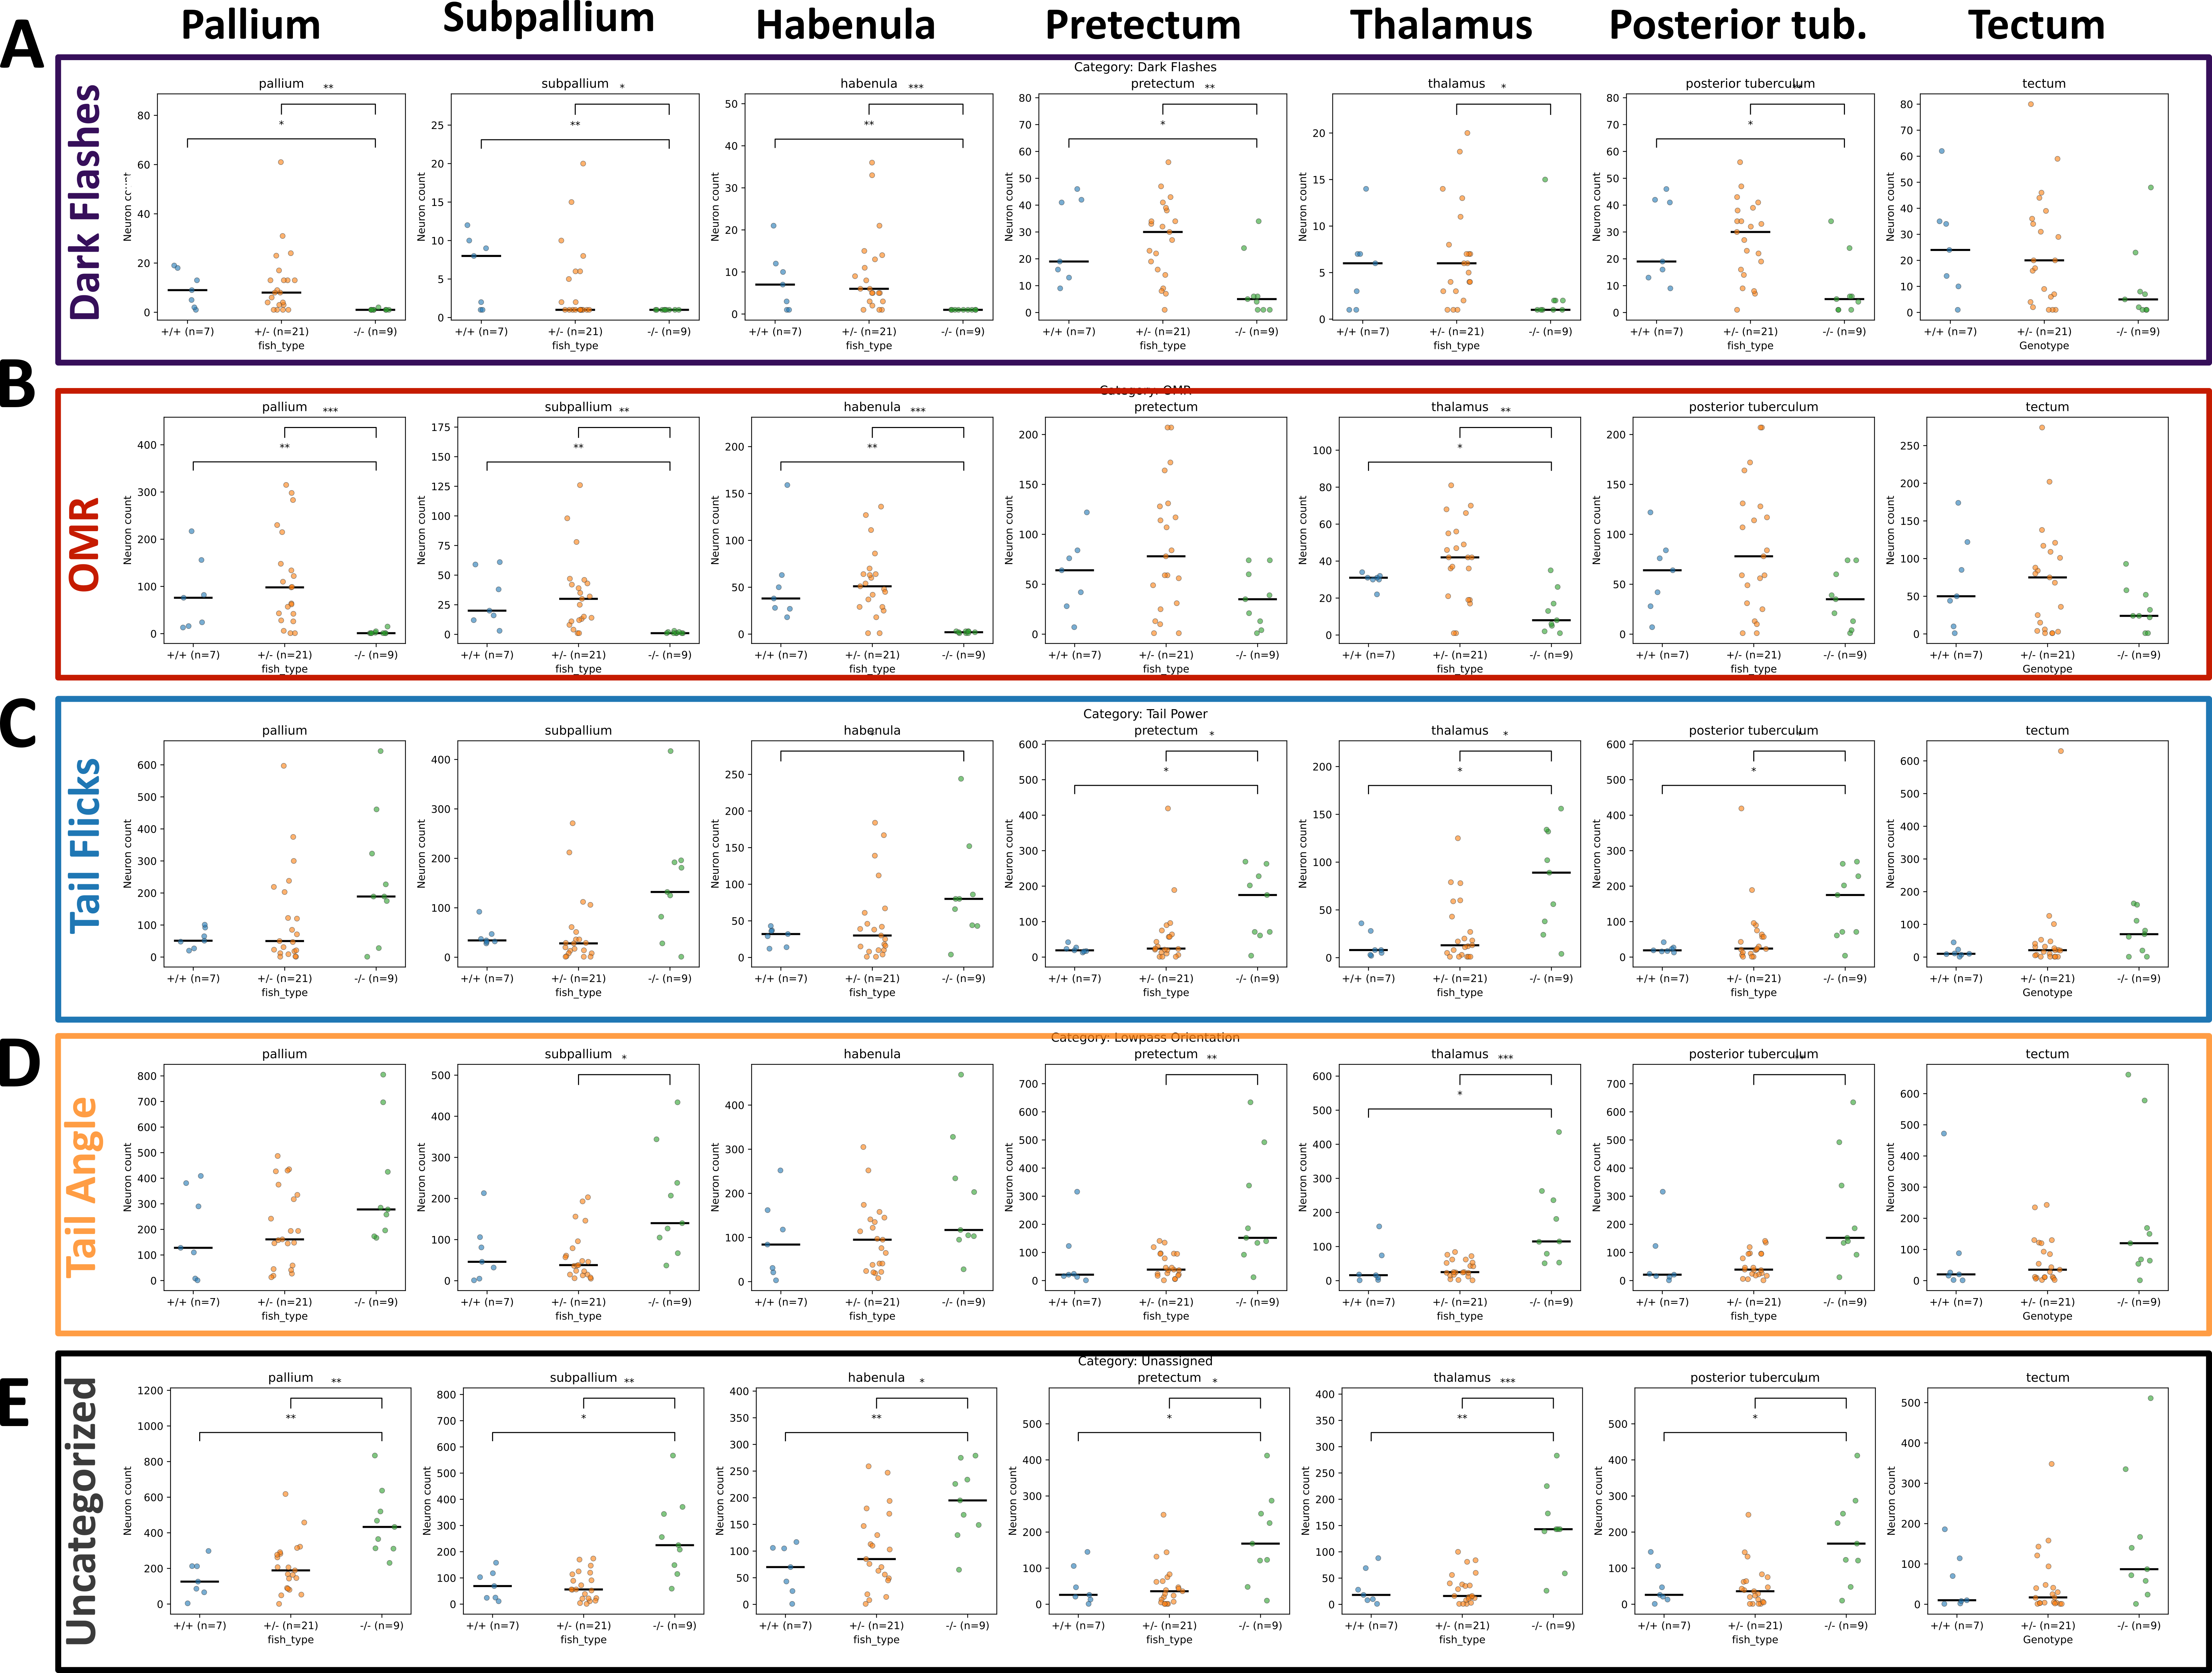
\includegraphics[width=0.9\linewidth]{Figures/SupplementartFig_RegionQuantification_Ca2Imaging.png}}
\label{fig:S_RegionQuant}

\figsupp[Activity heatmaps of \emph{atp1a3a} mutants, compared to heterozygous and wild-type siblings.]
{Activity heatmaps of \emph{atp1a3a} mutants, compared to heterozygous and wild-type siblings.
\textbf{A)}
}
{\includegraphics[width=0.9\linewidth]{Figures/SupplementartFig_Ca2Heatmaps.png}}

\label{fig:S_Ca2Heatmaps}

\end{center}
\end{figure}
\vspace{3mm}

While pERK is a very useful proxy for neuronal activity, it is an indirect measure that reflects the integrated activity of neurons over a timescale of minutes, and thus does not capture the fast dynamics of neural activity that are critical for sensorimotor processing.
To gain insight into the fast dynamics of neural activity in \emph{atp1a3a} mutants, we performed volumetric 2-photon Ca\textsuperscript{2+} imaging of the forebrain.
We crossed \emph{atp1a3a} mutants with a transgenic line that expresses the nuclear-targeted GCaMP6f Ca\textsuperscript{2+} indicator pan-neuronally, in the pigment deficient \emph{Nacre} mutants (\emph{Tg(elavl3:H2B-GCaMP6f); mitfa\textsuperscript{-/-}}), to generate a line that allows for brain-wide Ca\textsuperscript{2+} imaging in \emph{atp1a3a}. 

Larvae were imaged while head-embedded in agarose with the tail free to move and imaged with a modified \emph{pi\_tailtrack} apparatus \citep{Randlett2023}, integrating a video projector in order to present dynamic visual stimuli onto a screen below the larvae (\autoref{fig:6}A). Larvae were imaged over a 15-minute period, in a volume covering the areas of the forebrain showing the consistent altered activity patterns observed using pERK (\autoref{fig:5}, \autoref{fig:6}B). 
Larvae were presented with alternating DFs and 10 second pulses of forward OMR motion, repeated at 30 second intervals. 
This allowed us to compare how these stimuli are represented in forebrain neurons in the mutant brain, which we have established generate differential behavioural responses and pERK-derived activity patterns (\autoref{fig:2}, \autoref{fig:3}, \autoref{fig:4}). 

\subsubsection{Loss of sensory-tuned neurons in the atp1a3a mutant forebrain}

To analyze the Ca\textsuperscript{2+} imaging data, we segmented the imaging data into ROIs using suite2p \citep{Pachitariu2016}, which mostly (but not exclusively) identifies individual neuronal soma.
For simplicity, we refer to these ROIs as "neurons" here, though we acknowledge that some may be non-neuronal structures or multiple neurons within a single ROI.
Based on our MAP-Mapping results, we expected to see a reduction in sensory-related responses in \emph{atp1a3a} mutants, and indeed we saw significantly reduced numbers of DF and OMR responsive neurons in mutants relative to siblings (\autoref{fig:6}C-F).


Strikingly, there was a clear regional-dependence to this change, where the telencephalic pallium and subpallium, as well as the habenula showed a near complete loss of sensory-tuned neurons (\autoref{fig:S_RegionQuant}A,B).  
The other diencephalic regions we analyzed (pretectum, thalamus, posterior tuberculum) showed still strong but much less extreme reductions in these sensory-tuned neuronal populations. 
Our imaging volume also covered a portion of the midbrain tectum, which showed the least prominent reduction in sensory-tuned neurons, a difference which did not reach statistical significance. 

\subsubsection{Increase in motor-tuned neurons in the atp1a3a mutant forebrain}

As discussed above, in this head-embedded preparation, \emph{atp1a3a} mutants generally show a very bursty swimming pattern, interspersed with periods of persistent tail bends, with the tail often stably bent to one side for many seconds (\autoref{fig:1}F-I).
Therefore, we also attempted to identify neurons associated functionally with these abnormal motor patterns by identifying neurons tuned to swimming vigor, or longer-term dynamics in the average tail angle to capture this tail-bending phenotype.


In contrast to the reduced sensory-responsivness, our quantification of motor-related signals showed the opposite pattern, where we found significantly more neurons tuned to "swimming vigor" and "tail angle" in mutants relative to siblings (\autoref{fig:6}C,D,G,H).
This effect appeared to be relatively gloabal throughout the brain regions analyzed, but was most pronounced in the diencephalic regions (\autoref{fig:S_RegionQuant}C,D).
These data inidicate that the forebrain of \emph{atp1a3a} mutants isn't simply defective or hypo-responsive, but shows and imbalance of sensorimotor representation, with an increase in motor-realted signals and a reduction of sensory-tuned neurons. 

Understanding the neural basis of these complex swimming behaviour and postural bending phenotypes observed in these mutants will require a more global analysis of activity patterns, including in motor areas such as the hindbrain and spinal cord. 
How individual aberrant motor-events relate to identified neurons in the forebrain, and in particular the basal ganglia, will be of particular interest based on the known roles of these areas in motor control and action selection, and the strong alterations we observed in these areas in our MAP-Mapping experiments. 

\subsubsection{Abnormal bursting activity in atp1a3a mutant neurons}


Beyond a simple difference in the number of tuned neurons to motor-phenotypes, the nature of the activity pattern in these forebrain neurons was clearly very different in the mutants. 
In fact, this altered pattern is the most obvious and striking aspect of these data (\autoref{fig:S_Ca2Heatmaps}). 
Most of the functional categories of neurons that we identified as related to motor variables show a very bursty pattern of activity, with sustained periods of co-incident and persistent activity lasting many seconds to a few minutes, interspersed with longer periods of quiescence. 
Infact, most of these neurons were in the "active" phase of these bursts a single time during the course of the 15-minute imaging session, and thus show a very strong but transient pattern of activity that is not sustained across multiple bouts of swimming or tail bending.

This bursting pattern was also true of many classes of neurons for which we were not able to relate their activity to sensory or motor features, and were classified as "uncategorized", which represented a significantly larger population in the \emph{atp1a3a} mutants (\autoref{fig:6}C,D,I, \autoref{fig:S_RegionQuant}) indicating that this bursty pattern of activity may be a general feature of the mutant brain, at least across the areas we have observed here. Therefore, it is unclear if the correlation with motor variables is a direct relationship, or if these neurons are simply firing in their bursty activity pattern, the timing of which may correlate with motor phenotypes but not be involved in their generation. 
Determining this potentially causal relationship will likely require more detailed analysis of the timing and correlation of these bursting events, as well as direct interventions in the circuit (e.g. activation/suppression with holographic optogenetics).
In any case, such bursting activity rarely seen in wild-type or heterozygous siblings (\autoref{fig:S_Ca2Heatmaps}), and thus appears to be a very specific phenotype of the mutant forebrain.

\vspace{\baselineskip}
In summary, our Ca\textsuperscript{2+} imaging experiments have confirmed the hypothesis generated by our pERK experiments, where the \emph{atp1a3a} mutant forebrain, and in particular the habenula and tenelcephalon, exibit strongly altered physiology. This manifests as a strong bursting pattern of activity among many neurons within these (and adjacent) regions, as well as an imbalanced sensorimotor representation, with a reduction in sensory-tuned neurons and an increase in motor-related signals.


%%%%%%%% DISCUSSION: sensorimotor tuning %%%%%%%%
\subsubsection{Dysregulated sensorimotor tuning in the atp1a3a mutant forebrain}

To further investigate the effects of the \emph{atp1a3a} mutation on forebrain physiology, we used Ca\textsuperscript{2+} imaging to analyze the activity patterns of individual neurons, and to determine how sensory stimuli and motor responses are represented in these areas.
This revealed a strong reduction in the number of neurons that are tuned to both the DF and OMR stimuli. 
While this loss of functionally defined neurons was distributed across most brain areas we analyzed, it was most extreme in the areas implicted by our MAP-Mapping experiments: the pallium, subpallium and habenula. 
In these three brain areas WT and heterozygous controls had $\approx$10 and $\approx$100 neurons classified as DF and OMR tuned, respectively, while most mutants were completely devoid of these populations. 

This loss of sensory-tuning can not be explained simply by a lack of neuronal activity or generalized loss of tuning, as we observed an opposing pattern for the number of neurons that are tuned to motor variables -- either swimming vigor or the slower dymanics in the tail angle. This increas in motor-turning populations was observed consistently as a trend across all brain areas, but was most prominent in the diencephalon and did not reach statistical significance in the telencephalon and habenula. 
Similarly, the number of "uncategorized" neurons that were strongly active but not tuned to any of the sensory or motor variables we analyzed was significantly increased in mutants relative to siblings. 
Therefore, the mutant forebrain is not simply hypoactive or lacking in tuning, but shows a complex and region-specific pattern of imbalanced sensorimotor representation, with a reduction in sensory-tuned neurons and an increase in motor-related and unidentified signals.


%%%%%%%% DISCUSSION: bursting %%%%%%%%
\subsubsection{Abnormal bursting activity in the atp1a3a mutant forebrain}
When performing these analyses, our first-pass looks at the data using clustering visualization revealed a very striking pattern of altered bursting activity in the mutant forebrain, which was plainly visible in the raw data and was not present in wild-type or heterozygous siblings (as in \autoref{fig:S_Ca2Heatmaps}). 
This pattern consists of groups of neurons (tens to hundreds) showing prolonged periods of coincident and strong activity, bracketed by longer periods of quiescence.
While our anatomical analyses were limited to a relatively small volume of the brain, we did not see any clear regional specificity to this bursting pattern, which was observed across all the regions we analyzed, including the telencephalon and anterio-dorsal areas of the diencephalon and midbrain.

We note that these patterns are somewhat different and perhaps more dramatic than the differential activity patterns we observed in the MAP-Mapping experiments. 
As discussed above, this may be related to the behavioural contexts of freely-swimming vs. agarose head-embedded, the latter of which we hypothesize may trigger more pronounced phenotypes in a stress-dependent manner. 
Alternatively, this discrepancy may reflect differences in the temporal resolution of the methods, or the fact that ERK phosphorylation represents a complex intracellular proxy for neuronal activity. 
The MAPK/ERK pathway integrates synaptic inputs over time and responds differently to distinct temporal patterns of activity, which will likely differ substantially in the context of differet neuronal cell types, resulting in nonlinear and history-dependent signaling dynamics. 
Therefore, it is not actually clear how one might expect such a bursting pattern to manifest in an integrated pERK signal (increase or decrease relative to controls?), but our Ca\textsuperscript{2+} imaging results clearly confirm that the areas implicated by MAP-Mapping show stronlgy altered physiology in the mutant brain. 

This bursting pattern is particularly interesting in the context of the observed altered cortical physiology in ATP1A3-related disorders and model systems. 
In particular, we note the potential similarities between this phenotype of sparse but seemingly uncontrolled busts of activity in populations of neurons, and the quasi-epiliptic phenomena associated with ATP1A3-loss, including the cortical spreading depolarizations that have been observed in mouse models of ATP1A3-related disorders, which are thought to be related to the paroxysmal symptoms  \citep{Hunanyan2014, Balestrino1999}.
Spreading depolarization are a slowly propagating wave of near-complete neuronal depolarization followed by prolonged synaptic silencing \citep{Dreier2011}.
Because recovery from spreading depolarization critically depends on Na$^+$/K$^+$-ATPase activity, ATP1A3 dysfunction is predicted to lower the threshold for SD initiation and prolong recovery \citep{Hunanyan2014, Balestrino1999}.
This framework accounts for the defining features of hemiplegic episodes, including abrupt onset, reversibility, sleep-related resolution, and alternating laterality across attacks.
 
Further characterization of the cell-type specific characteristics of these bursting activty patterns, their spatial and temporal dynamics, as well as their relationship to motor phenotypes and with stress-based triggers, will be important next steps in understanding the pathophysiology of ATP1A3 loss and its relationship to the paroxysmal symptoms of ATP1A3-related disorders.
This insight may provide an important high-throughput model system for screening for interventions (such as high-oxygen treatment, \citealp{Papadopoulou2023_MD}) that can suppress these abnormal activity patterns. 
